\let\negmedspace\undefined
\let\negthickspace\undefined
\documentclass[journal,12pt,onecolumn]{IEEEtran}
\usepackage{cite}
\usepackage{amsmath,amssymb,amsfonts,amsthm}
\usepackage{algorithmic}
\usepackage{graphicx}
\graphicspath{{./figs/}}
\usepackage{textcomp}
\usepackage{xcolor}
\usepackage{txfonts}
\usepackage{listings}
\usepackage{enumitem}
\usepackage{mathtools}
\usepackage{gensymb}
\usepackage{comment}
\usepackage{caption}
\usepackage[breaklinks=true]{hyperref}
\usepackage{tkz-euclide} 
\usepackage{listings}
\usepackage{gvv}                                        
%\def\inputGnumericTable{}                                 
\usepackage[latin1]{inputenc}     
\usepackage{xparse}
\usepackage{color}                                            
\usepackage{array}
\usepackage{longtable}                                       
\usepackage{calc}                                             
\usepackage{multirow}
\usepackage{multicol}
\usepackage{hhline}                                           
\usepackage{ifthen}                                           
\usepackage{lscape}
\usepackage{tabularx}
\usepackage{array}
\usepackage{float}
\usepackage{parskip}
\newtheorem{theorem}{Theorem}[section]
\newtheorem{problem}{Problem}
\newtheorem{proposition}{Proposition}[section]
\newtheorem{lemma}{Lemma}[section]
\newtheorem{corollary}[theorem]{Corollary}
\newtheorem{example}{Example}[section]
\newtheorem{definition}[problem]{Definition}
\newcommand{\BEQA}{\begin{eqnarray}}
\newcommand{\EEQA}{\end{eqnarray}}
\newcommand{\define}{\stackrel{\triangle}{=}}
\theoremstyle{remark}
\newtheorem{rem}{Remark}

\begin{document}
\title{2.10.73}
\author{EE25BTECH11045 - P.Navya Priya}
\maketitle
\renewcommand{\thefigure}{\theenumi}
\renewcommand{\thetable}{\theenumi}

\textbf{Question:}

 Let $\vec{A}$, $\vec{B}$ and $\vec{C}$ be unit vectors. Suppose that  $\vec{A}\cdot\vec{B}$ =  $\vec{A}\cdot\vec{C}$= 0, and that the angle between  $\vec{B}$ and  $\vec{C}$ is $\frac{\pi}{6}$. Then $\vec{A}= \pm2(\vec{B}\times\vec{C})$
 \vspace{0.5cm}

\textbf{Solution:}

Let us solve the given equation theoretically and then verify the solution computationally.\\

Since $\vec{A}\cdot\vec{B}$ =  $\vec{A}\cdot\vec{C}$= 0, it follows that $\vec{A}$ is perpendicular to both $\vec{B}$ and $\vec{C}$. Therefore A is parallel(or anti-parallel) to the cross product of $\vec{B}$ and $\vec{C}$.

\begin{align}
    \vec{A}\,=\,\lambda(\vec{B}\times\vec{C})
\end{align}
From the given question,
\begin{align}
    \vec{B}^\top\vec{C}=\text{cos}\brak{\frac{\pi}{6}}
\end{align}
We know that,
\begin{align}
 \vec{B}^\top\vec{C}^{2}\,+\,||\vec{B}\times\vec{C}||^{2}=||\vec{B}||^{2}||\vec{C}||^{2}
\end{align}
\begin{align}
 \implies   ||\vec{B}\times\vec{C}||^{2}\,=\,\frac{1}{4}
\end{align}
\begin{align}
   \implies   ||\vec{B}\times\vec{C}||\,=\,\frac{1}{2}
\end{align}
As $\vec{A}$ is a unit vector,\\
from(1)
\begin{align}
    ||\vec{A}||\,=\,||\lambda(\vec{B}\times\vec{C})||
\end{align}
\begin{align}
    1\,=\,|\lambda|\frac{1}{2}
\end{align}
Hence

\begin{align}
 \lambda\,=\,\pm 2
\end{align}

\begin{align}
    \therefore \vec{A}\,=\,\pm 2(\vec{B}\times\vec{C})
\end{align}
\newpage
To verify the solution computationally let us assume the vectors $\vec{B}$ and $\vec{C}$ as 

\centering
$\vec{B}=\myvec{1\\0\\0}$ and $\vec{C}=\myvec{\frac{\sqrt{3}}{2}\\[4pt]\frac{1}{2}\\0}$

\begin{figure}[H]
\centering
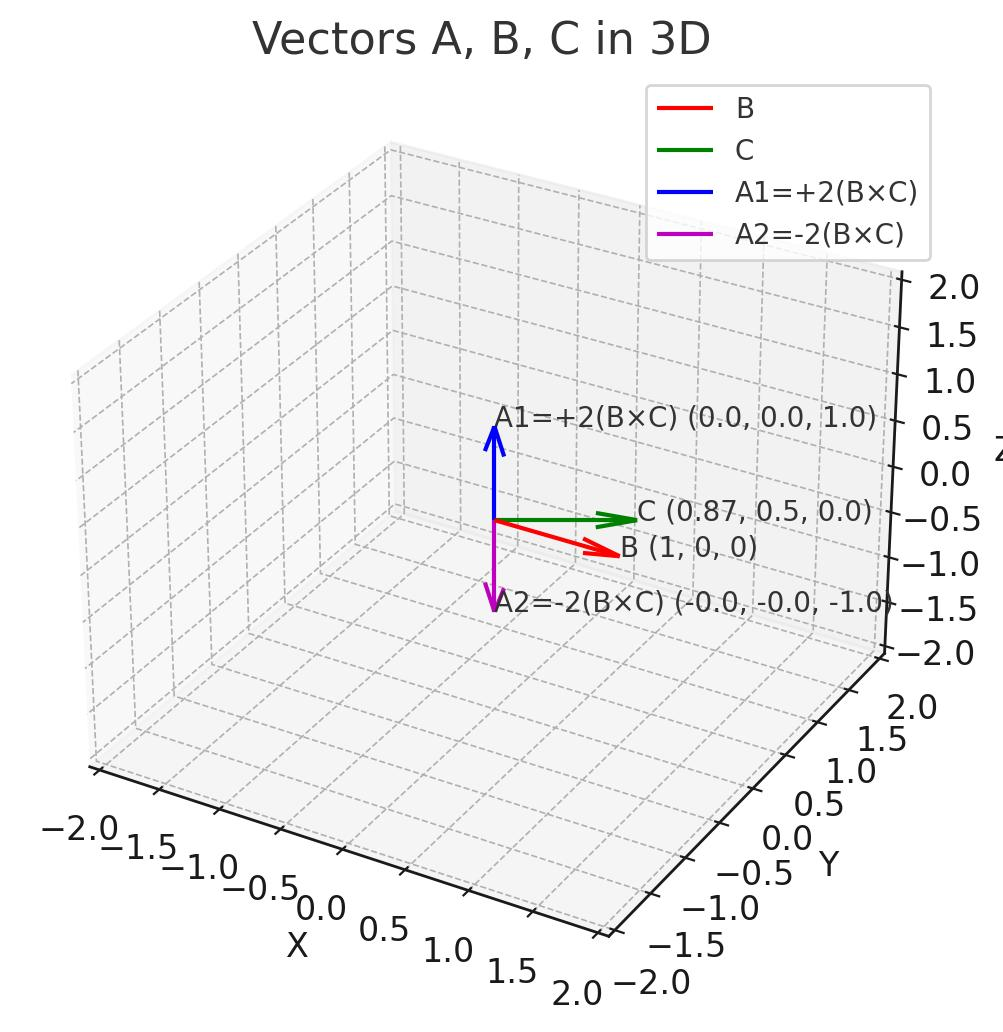
\includegraphics[width=0.7\columnwidth]{figs/graph.png}
\label{fig:graph.png}
\end{figure}
\end{figure}
\end{document}



































